% CH4114 — Tutorial 00, Part 1: Git & GitHub
% Beamer deck, 16:9, compiled with pdflatex (TeX Live 2026)
% Author: Shuvam Banerji Seal
\documentclass[aspectratio=169]{beamer}

\usetheme{Madrid}
\usecolortheme{whale}
\setbeamertemplate{navigation symbols}{}

\usepackage[T1]{fontenc}
\usepackage{tikz}
\usetikzlibrary{arrows.meta, positioning}
\usepackage{booktabs}
\usepackage{listings}
\lstset{
  basicstyle=\ttfamily\footnotesize,
  breaklines=true,
  showstringspaces=false,
  columns=fullflexible,
  keepspaces=true,
}

\title[Git \& GitHub]{Tutorial 00 --- Part 1\\[2pt] Git \& GitHub}
\subtitle{Version control for research code}
\author[SBS]{Shuvam Banerji Seal}
\institute[CH4114]{CH4114 --- Molecular Simulation}
\date[Aug 2026]{14 August 2026}

\begin{document}

% ------------------------------------------------------------------ title
\begin{frame}[plain]
  \titlepage
  \centering{\scriptsize Course Instructor: Dr.\ Susmita Roy \quad$\cdot$\quad TA: Shuvam Banerji Seal}\par
  \vspace{0.1cm}
  \centering{\scriptsize Repository: \texttt{CH4114\_Molecular\_Simulation\_Tutorials}}
\end{frame}

\section{Why version control}

% ------------------------------------------------------------ motivation
\begin{frame}{Why version control?}
  \begin{itemize}
    \item Research code evolves: \texttt{analysis\_final.py},
          \texttt{analysis\_final\_v2.py}, \texttt{analysis\_FINAL\_v3.py}\ldots
    \item Without history, a deleted good version is \textbf{gone forever}.
    \item Simulations are \textbf{reproducible} only if the code is versioned
          and taggable.
  \end{itemize}
  \vspace{0.3cm}
  \begin{block}{The promise of Git}
    Complete history of every change, instant undo, safe experiments on
    branches, clean multi-person collaboration, and a snapshot you can cite.
  \end{block}
\end{frame}

% --------------------------------------------------------------- benefits
\begin{frame}{What Git gives you}
  \begin{table}
    \small
    \begin{tabular}{@{}ll@{}}
      \toprule
      Superpower & Why it matters for simulation work \\
      \midrule
      History & See exactly what changed, when, and by whom \\
      Undo & Revert to any past state of your code \\
      Branches & Try a new idea without breaking working code \\
      Collaboration & Merge work from multiple people cleanly \\
      Reproducibility & Tag a commit = a snapshot you can share \\
      \bottomrule
    \end{tabular}
  \end{table}
  \vspace{0.3cm}
  \begin{itemize}
    \item Git takes \textbf{snapshots} (commits) of your project.
    \item Each commit is cheap, local, and complete.
  \end{itemize}
\end{frame}

% ------------------------------------------------------------ mental model
\begin{frame}{The mental model: three areas}
  \begin{center}
    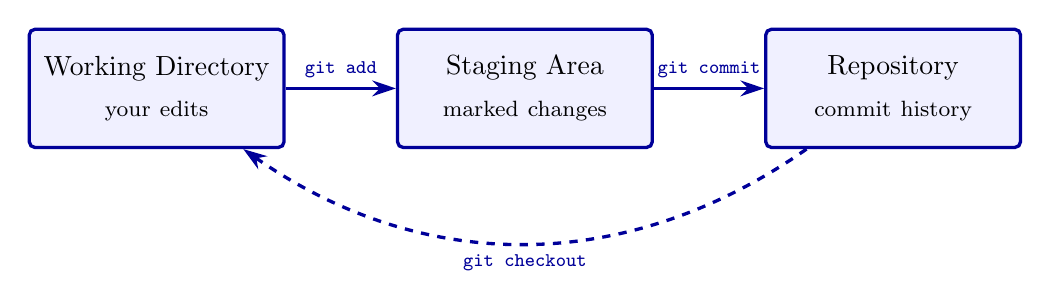
\begin{tikzpicture}[
        box/.style={rectangle, draw=blue!60!black, very thick,
                    rounded corners=2pt, fill=blue!6, text width=3.0cm,
                    align=center, minimum height=1.5cm},
        lab/.style={font=\scriptsize\ttfamily, text=blue!60!black},
        arr/.style={-{Stealth[length=3mm,width=2mm]}, very thick, blue!60!black},
        node distance=1.4cm]
      \node[box] (wd) {Working Directory\\[3pt] {\footnotesize your edits}};
      \node[box, right=of wd] (st) {Staging Area\\[3pt] {\footnotesize marked changes}};
      \node[box, right=of st] (rp) {Repository\\[3pt] {\footnotesize commit history}};
      \draw[arr] (wd) -- node[lab, above] {git add} (st);
      \draw[arr] (st) -- node[lab, above] {git commit} (rp);
      \draw[arr, dashed, bend left=35] (rp) to node[lab, below] {git checkout} (wd);
    \end{tikzpicture}
  \end{center}
  \vspace{0.3cm}
  \begin{itemize}
    \item \textbf{Working directory} --- files you are editing.
    \item \textbf{Staging area} --- changes marked for the next snapshot.
    \item \textbf{Repository} --- all committed snapshots (the history).
  \end{itemize}
\end{frame}

% --------------------------------------------------------------- workflow
\begin{frame}[fragile]{The core workflow}
  \begin{columns}[T]
    \begin{column}{0.48\textwidth}
      \begin{block}{The loop (memorize it)}
        \begin{lstlisting}
git init          # once
git status        # what changed?
git add <file>    # stage changes
git commit -m "msg"
        \end{lstlisting}
      \end{block}
    \end{column}
    \begin{column}{0.48\textwidth}
      \begin{itemize}
        \item Commit after every \textbf{meaningful} chunk of work.
        \item Run \texttt{git status} constantly.
        \item Write commit messages that explain \emph{why}.
      \end{itemize}
      \vspace{0.3cm}
      \begin{alertblock}{Rule}
        Working LJ potential script = commit.
        Every keystroke = no.
      \end{alertblock}
    \end{column}
  \end{columns}
\end{frame}

% ------------------------------------------------------ config and history
\begin{frame}[fragile]{First-time config and history}
  \begin{columns}[T]
    \begin{column}{0.48\textwidth}
      \begin{block}{One-time setup (per machine)}
        \begin{lstlisting}
git config --global user.name  "You"
git config --global user.email "you@x.com"
git config --global init.defaultBranch main
        \end{lstlisting}
      \end{block}
    \end{column}
    \begin{column}{0.48\textwidth}
      \begin{block}{Inspecting history}
        \begin{lstlisting}
git log --oneline
git log --oneline --graph
git status
git diff
git diff --staged
        \end{lstlisting}
      \end{block}
    \end{column}
  \end{columns}
\end{frame}

% ------------------------------------------------------------------ undo
\begin{frame}{Undoing changes: three levels}
  \begin{table}
    \small
    \begin{tabular}{@{}lll@{}}
      \toprule
      Situation & Command & Effect \\
      \midrule
      Edited, not staged & \texttt{git restore <file>} & discard edits \\
      Staged by mistake & \texttt{git restore --staged <file>} & unstage, keep edits \\
      Wrong commit message & \texttt{git commit --amend -m "msg"} & rewrite last commit \\
      \bottomrule
    \end{tabular}
  \end{table}
  \vspace{0.4cm}
  \begin{block}{Safety}
    Git never throws work away silently --- \texttt{git restore} only touches
    what you point it at. When in doubt, commit first, clean up later.
  \end{block}
\end{frame}

% -------------------------------------------------------------- branching
\begin{frame}{Branching and merging}
  \begin{center}
    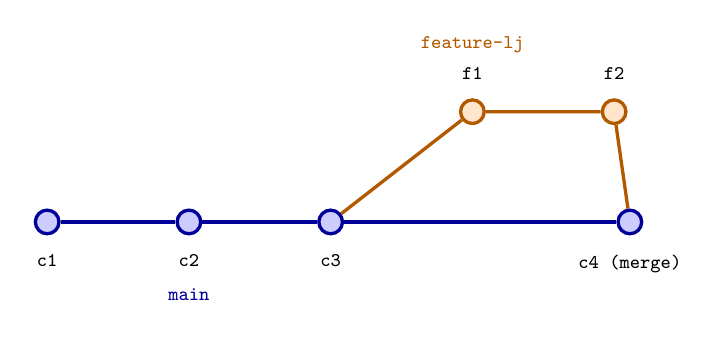
\begin{tikzpicture}[
        mc/.style={circle, draw=blue!60!black, very thick, fill=blue!20,
                   minimum size=0.30cm, inner sep=0pt},
        fc/.style={circle, draw=orange!70!black, very thick, fill=orange!20,
                   minimum size=0.30cm, inner sep=0pt},
        lab/.style={font=\scriptsize\ttfamily}]
      \node[mc] (c1) at (0,0) {};
      \node[mc] (c2) at (1.8,0) {};
      \node[mc] (c3) at (3.6,0) {};
      \node[mc] (c4) at (7.4,0) {};
      \draw[very thick, blue!60!black] (c1) -- (c2) -- (c3) -- (c4);
      \node[fc] (f1) at (5.4,1.4) {};
      \node[fc] (f2) at (7.2,1.4) {};
      \draw[very thick, orange!70!black] (c3) -- (f1) -- (f2) -- (c4);
      \node[lab, below=0.12cm of c1] {c1};
      \node[lab, below=0.12cm of c2] {c2};
      \node[lab, below=0.12cm of c3] {c3};
      \node[lab, below=0.12cm of c4] {c4 (merge)};
      \node[lab, above=0.12cm of f1] {f1};
      \node[lab, above=0.12cm of f2] {f2};
      \node[lab, below=0.55cm of c2, text=blue!60!black] {main};
      \node[lab, above=0.45cm of f1, text=orange!70!black] {feature-lj};
    \end{tikzpicture}
  \end{center}
  \vspace{0.2cm}
  \begin{itemize}
    \item \texttt{main} stays clean; experiments live on short-lived branches.
    \item \texttt{git merge feature-lj} folds the branch back in.
    \item Golden rule: never develop directly on \texttt{main}.
  \end{itemize}
\end{frame}

% ---------------------------------------------------------------- conflict
\begin{frame}[fragile]{Merge conflicts}
  Happen when two branches edit the same lines. Git marks them:
  \begin{block}{conflict markers in the file}
    \begin{lstlisting}
<<<<<<< HEAD
E = 4 * eps * ((sigma/r)**12 - (sigma/r)**6)
=======
E = eps * ((sigma/r)**12 - (sigma/r)**6)
>>>>>>> feature-lj
    \end{lstlisting}
  \end{block}
  \begin{enumerate}
    \item Edit the file by hand --- keep the correct version.
    \item \texttt{git add <file>}
    \item \texttt{git commit -m "resolve merge conflict"}
  \end{enumerate}
\end{frame}

\section{GitHub}

% --------------------------------------------------------------- github
\begin{frame}{GitHub: hosting, sharing, collaborating}
  \begin{table}
    \small
    \begin{tabular}{@{}ll@{}}
      \toprule
      Element & Purpose \\
      \midrule
      Code & browse files and commit history \\
      Issues & bug reports, feature requests, task tracking \\
      Pull requests & propose and review changes before merging \\
      Actions & CI/CD: run tests automatically on every push \\
      README & the front page of your project \\
      \bottomrule
    \end{tabular}
  \end{table}
  \vspace{0.3cm}
  \begin{itemize}
    \item GitHub is a \textbf{hosting service} for Git repositories.
    \item Cloud backup + collaboration hub + public portfolio.
  \end{itemize}
\end{frame}

% ------------------------------------------------------------- remote
\begin{frame}{Local repository $\leftrightarrow$ GitHub}
  \begin{center}
    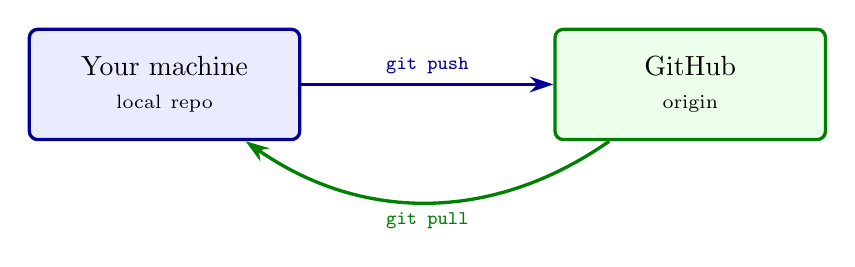
\begin{tikzpicture}[
        loc/.style={rectangle, draw=blue!60!black, very thick,
                    rounded corners=3pt, fill=blue!8, text width=3.2cm,
                    align=center, minimum height=1.4cm},
        rem/.style={rectangle, draw=green!50!black, very thick,
                    rounded corners=3pt, fill=green!8, text width=3.2cm,
                    align=center, minimum height=1.4cm},
        arr/.style={-{Stealth[length=3mm,width=2mm]}, very thick},
        node distance=3.2cm]
      \node[loc] (l) {Your machine\\ {\scriptsize local repo}};
      \node[rem, right=of l] (r) {GitHub\\ {\scriptsize origin}};
      \draw[arr, blue!60!black] (l) -- node[above, font=\scriptsize\ttfamily] {git push} (r);
      \draw[arr, green!50!black, bend left=35] (r) to node[below, font=\scriptsize\ttfamily] {git pull} (l);
    \end{tikzpicture}
  \end{center}
  \vspace{0.3cm}
  \begin{itemize}
    \item \texttt{git remote add origin <url>} --- connect once.
    \item \texttt{git push -u origin main} --- first push; afterwards plain \texttt{git push}.
    \item \texttt{git clone <url>} --- copy a remote repo to your machine.
  \end{itemize}
\end{frame}

% ------------------------------------------------------------ collaboration
\begin{frame}{Collaboration loop: issues, branches, pull requests}
  \begin{enumerate}
    \item Open an \textbf{issue} describing the task.
    \item Create a branch: \texttt{git checkout -b fix-lj-preprint}
    \item Commit and push: \texttt{git push -u origin fix-lj-preprint}
    \item Open a \textbf{pull request} on GitHub: ``Closes \#12 --- fixes LJ prefactor''.
    \item Reviewer comments; push more commits; \textbf{merge}.
    \item Pull locally: \texttt{git pull}
  \end{enumerate}
  \vspace{0.3cm}
  \begin{block}{Why PRs?}
    Nothing lands on \texttt{main} unreviewed --- history records intent.
  \end{block}
\end{frame}

% ------------------------------------------------------------------ gh
\begin{frame}[fragile]{The gh CLI: GitHub from your terminal}
  \begin{block}{Authenticate once}
    \begin{lstlisting}
gh auth login
gh auth status
    \end{lstlisting}
  \end{block}
  \begin{block}{Daily commands}
    \begin{lstlisting}
gh repo create my-repo --public --source . --push
gh issue create --title "Add MC code" --body "..."
gh pr create --title "..." --body "..."
gh repo view --web
    \end{lstlisting}
  \end{block}
  \begin{itemize}
    \item \texttt{gh repo create --source . --push} is exactly how this
          repository was published.
  \end{itemize}
\end{frame}

% ------------------------------------------------------------- cheat sheet
\begin{frame}[fragile]{Cheat sheet --- print this}
  \begin{columns}[T]
    \begin{column}{0.48\textwidth}
      \begin{lstlisting}[basicstyle=\ttfamily\scriptsize]
# setup
git config --global user.name "N"
git config --global user.email "e"

# everyday
git status
git diff
git log --oneline
git add <file> | git add .
git commit -m "msg"
git push | git pull

# branches
git branch <name>
git checkout -b <name>
git switch <name>
git merge <name>
git branch -d <name>
      \end{lstlisting}
    \end{column}
    \begin{column}{0.48\textwidth}
      \begin{lstlisting}[basicstyle=\ttfamily\scriptsize]
# undo
git restore <file>
git restore --staged <file>
git commit --amend -m "msg"

# remote
git remote -v
git remote add origin <url>
git clone <url>

# github
gh auth login
gh repo create NAME --public \
   --source . --push
gh pr create
gh issue create
      \end{lstlisting}
    \end{column}
  \end{columns}
\end{frame}

% ------------------------------------------------------------ check yourself
\begin{frame}{Check yourself}
  \begin{enumerate}
    \item What is the difference between \texttt{git add} and \texttt{git commit}?
    \item A collaborator changed \texttt{main} while you worked on a branch.
          Which two commands bring their changes in?
    \item You committed with a typo'd message. Which one command fixes it?
    \item Which command creates a GitHub repository from the current folder
          and pushes it?
  \end{enumerate}
  \vspace{0.4cm}
  \begin{block}{Next up}
    Part 2: organizing your project like a professional. \quad
    Part 3: uv environments.
  \end{block}
\end{frame}

\end{document}
